\section{Analysis}
\label{sec:theory}


%\newenvironment{claim}[1]{\par\noindent\underline{Claim:}\space#1}{}
\newenvironment{claimproof}[1]{\par\noindent\underline{Proof:}\space#1}{\hfill $\blacksquare$}

%\newtheorem{problem}{Problem}

%% \theoremstyle{definition}
%% \newtheorem{definition}{Definition}[section]

%% \theoremstyle{theorem}
%% \newtheorem{theorem}{Theorem}[section]

%% \theoremstyle{lemma}
%% \newtheorem{lemma}{Lemma}[section]

\newcommand{\bigo}{\mathcal{O}}
\newcommand{\page}{\pi}
\newcommand{\str}{s}
\newcommand{\node}{\mathit {v}}
\newcommand{\W}{\mathcal {W}}
\newcommand{\lp}{\left(}
%\newcommand{\rparen}{\right)}
\newcommand{\rparen}{\right)}
\newcommand{\rp}{\right)}

%%caveat required for lemma 4.4 added below.  run by andrew before finalizing
This section shows that the \sm procedure described in
\S\ref{sec:meshing-algorithm} comes with strong formal guarantees on
the \textit{quality} of the meshing found along with bounds on its
\textit{runtime}.  In situations where significant meshing
opportunities exist (that is, when compaction is most desirable), \sm
finds with high probability an approximation arbitrarily close to
$1/2$ of the best possible meshing in $O\lp n/q\rparen$ time, where
$n$ is the number of spans and $q$ is the global probability of two
spans meshing.

To formally establish these bounds on quality and runtime, we show
that meshing can be interpreted as a graph problem, analyze its
complexity (\S\ref{subsec:graph}), show that we can do nearly as well
by solving an easier graph problem instead (\S\ref{subsec:matching}),
and prove that \sm approximates this problem with high probability
(\S\ref{subsec:analysis}).

% \item{Introduce an easily-computable \emph{a priori} lower bound for the effect of meshing (\S\ref{subsec:lowerbound})}
%\end{itemize}

\begin{figure}[!t]
  \centering
  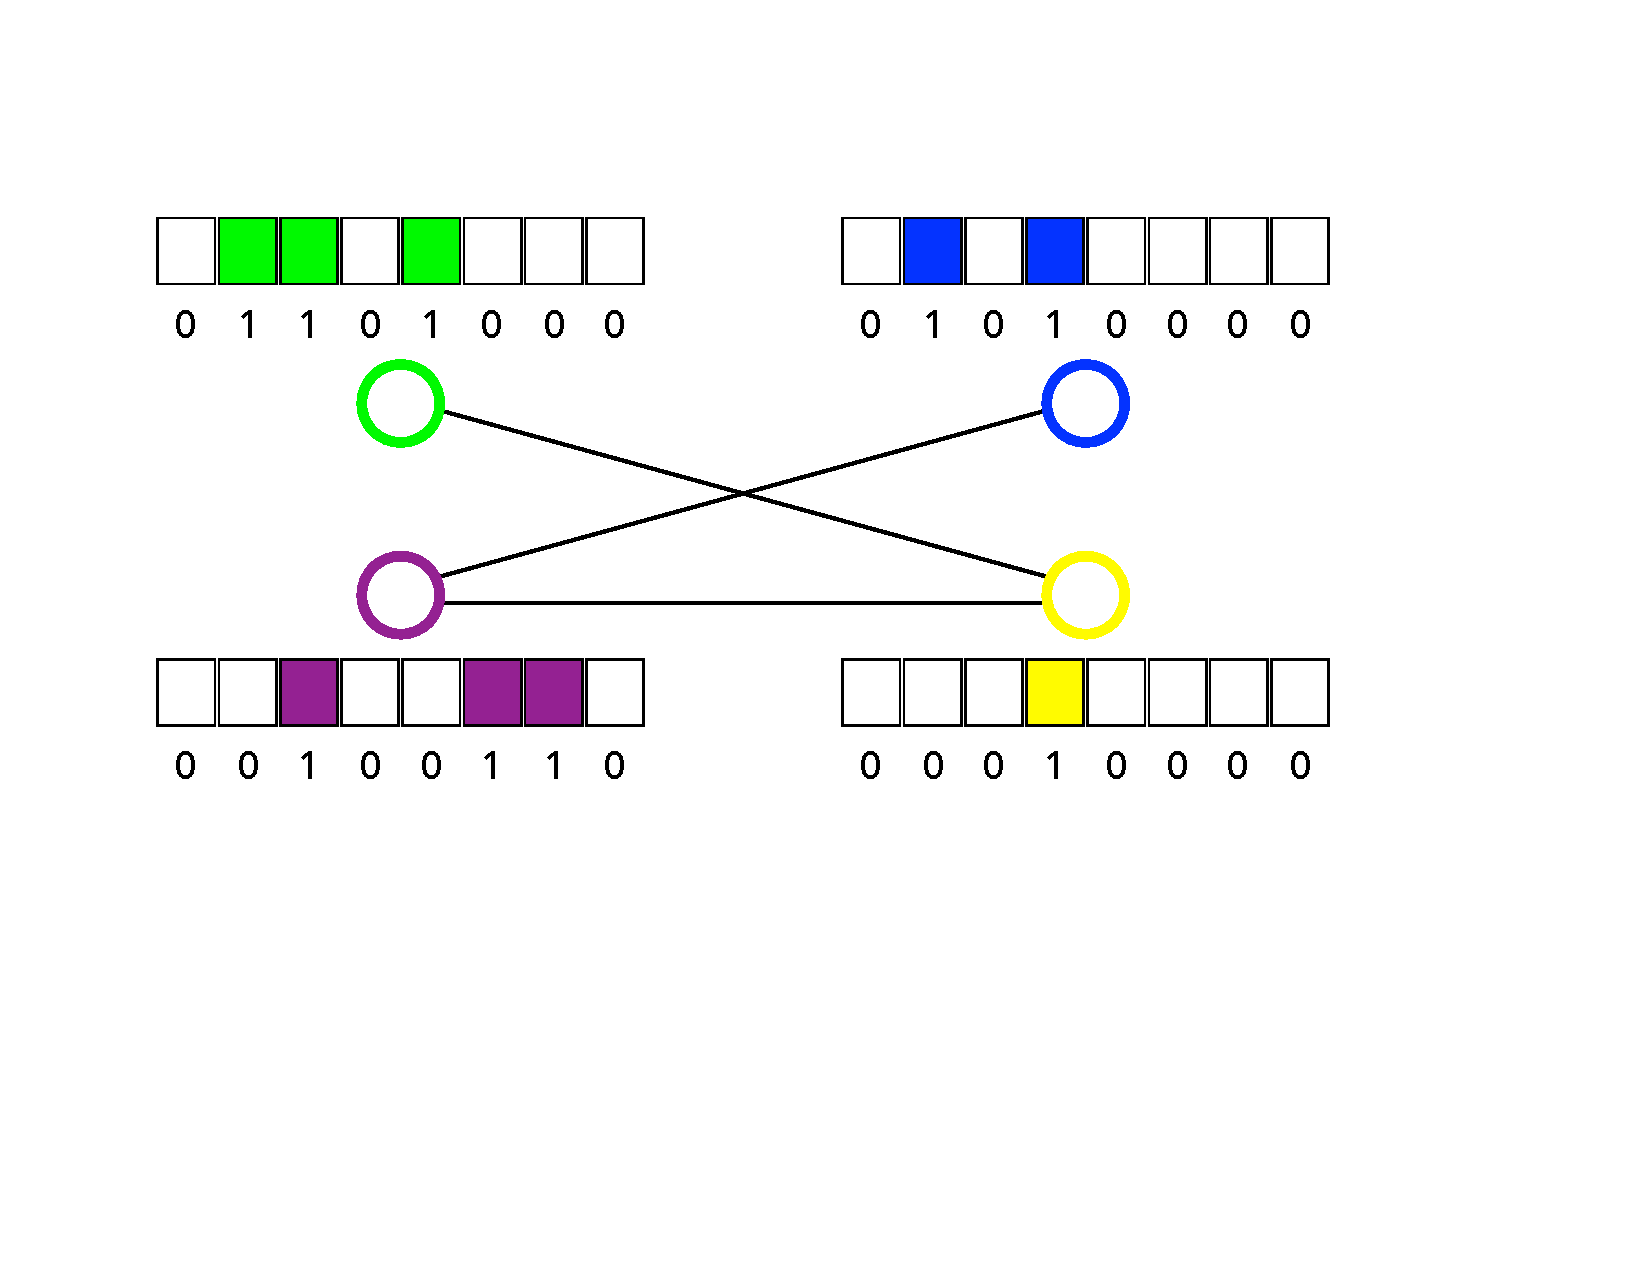
\includegraphics[width=.8\textwidth]{Chapters/mesh/figures/graph-diagram.pdf}
%  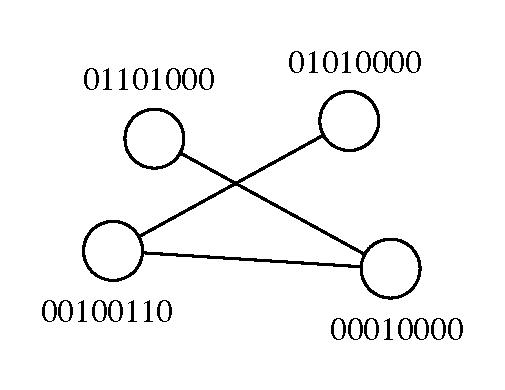
\includegraphics[width=.33\textwidth]{figures/meshing_graph.pdf}
%  \vspace{-2em}
%\centering
\caption{\textbf{An example meshing graph.}  Nodes correspond to the spans represented by the strings \texttt{01101000}, \texttt{01010000}, \texttt{00100110}, and \texttt{00010000}.  Edges connect meshable strings (corresponding to non-overlapping spans).}\label{fig:exmesh}
\end{figure}


\subsection{Formal Problem Definitions}
\label{subsec:probdef}
Since \Mesh{} segregates objects based on size, we can limit our
analysis to compaction within a single size class without loss of
generality. For our analysis, we represent spans as binary strings of
length $b$, the maximum number of objects that the span can
store. Each bit represents the allocation state of a single object. We
represent each span $\page$ with string $\str$ such that $\str\lp
i\rparen = 1$ if $\page$ has an object at offset $i$, and 0 otherwise.

\begin{definition}
We say  two  strings $\str_{1}, \str_{2}$ \em{mesh} iff $\sum_i \str_{1}\lp i\rparen \cdot \str_{2} \lp i \rparen = 0$. More generally, a set of binary strings are said to mesh if every pair of strings in this set mesh.
%We say that k binary strings $\str_{1}, ... \str_{k}$ mesh iff $\sum_{j \in [1,k]} \str_{j}(i) \leq 1$ $\forall i \in [0,b-1]$.\\
%Equivalently, k binary strings mesh if each each of said strings are pairwise meshable with all of the other strings.
\end{definition}

When we mesh $k$ spans together, the objects scattered across those
$k$ spans are moved to a single span while retaining their offset from
the start of the span. The remaining $k-1$ spans are no longer needed
and are released to the operating system. We say that we ``release''
$k-1$ \emph{strings} when we mesh $k$ strings together.  Since our
goal is to empty as many physical spans as possible, we can
characterize our theoretical problem as follows:

\begin{problem}
Given a multi-set of $n$ binary strings of length $b$, find a meshing
that releases the maximum number of strings.
\end{problem}

% Note that the total number of strings released is equal to $n - \rho -
% \phi$, where $\rho$ is the number of total meshes performed, and $\phi$
% is the number of strings that remain unmeshed.

\paragraph*{A Formulation via Graphs:}
\label{subsec:graph}

We observe that an instance of the meshing problem, a string multi-set
$S$, can naturally be expressed via a graph $G(S)$ where there is a
node for every string in $S$ and an edge between two nodes iff the
relevant strings can be meshed. Figure~\ref{fig:exmesh} illustrates
this representation via an example.

%Given , we construct a meshing graph $G_S$ as follows:\\
%We add a node $\node$ to $G_S$ for each $\str \in S$.  We say node $\node$ represents $\str$.  For each %node pair $\node_1, \node_2$, we add edge $(\node_1, \node_2)$ iff $\node_1$ and $\node_2$ mesh.

%This meshing problem is reducible to min clique cover (MCC), an NP-Complete problem.  We implicitly show %this reduction through a straightforward graph interpretation of the meshing problem.

If a set of strings are meshable, then there is an edge between every
pair of the corresponding nodes: the set of corresponding nodes is a
\emph{clique}. We can therefore decompose the graph into $k$ disjoint
cliques iff we can free $n-k$ strings in the meshing
problem. Unfortunately, the problem of decomposing a graph into the
minimum number of disjoint cliques (\textsc{MinCliqueCover}) is in
general NP-hard. Worse, it cannot even be approximated up to a factor
$m^{1-\epsilon}$ unless $P=NP$~\cite{zuckerman07}.

While the meshing problem is reducible to {\textsc{MinCliqueCover}},
we have not shown that the meshing problem is NP-Hard.  The meshing
problem is indeed NP-hard for strings of arbitrary length, but in
practice string length is proportional to span size, which is
constant.

\begin{theorem}\label{thm:polytime}
The meshing problem for $S$, a multi-set of strings of constant length, is in $P$. %can be solved in polynomial time.
%is in P
%; equivalently, the min clique cover problem on meshing graphs generated from sets of strings of constant %length is in P.
\end{theorem}

\begin{proof}
We assume without loss of generality that $S$ does not contain the
all-zero string $\str_0$; if it does, since $\str_0$ can be meshed
with any other string and so can always be released, we can solve the
meshing problem for $S \setminus \str_0$ and then mesh each instance
of $\str_0$ arbitrarily.

Rather than reason about {\textsc{MinCliqueCover}} on a
 meshing graph $G$, we consider the equivalent
problem of coloring the complement graph $\bar{G}$ in which there is
an edge between every pair of two nodes whose strings do not mesh. The nodes of $\bar{G}$ can be partitioned into at most $2^b-1$
subsets $N_1 \ldots N_{2^b-1}$ such that all nodes in each
$N_i$ represent the same string $\str_i$.  The induced subgraph of
$N_i$ in $\bar{G}$ is a clique since all its nodes have a 1 in the same position and so cannot be pairwise meshed.  Further, all nodes in $N_i$ have the same set of neighbors.

Since $N_i$ is a clique, at most one node in $N_i$ may be colored with
any color.  Fix some coloring on $\bar{G}$.  Swapping the colors of
two nodes in $N_i$ does not change the validity of the coloring since
these nodes have the same neighbor set.  We can therefore
unambiguously represent a valid coloring of $\bar{G}$ merely by
indicating in which cliques each color appears.

With $2^b$ cliques and a maximum of $n$ colors, there are at most $\lp
n+1 \rparen ^{c}$ such colorings on the graph where $c=2^{2^b}$. This follows because each color used can be associated with a subset of $\{1, \ldots, 2^b\}$ corresponding to which of the cliques have node with this color; we call this subset a \emph{signature} and note there are $c$ possible signatures. A coloring can be therefore be associated with a multi-set of possible signatures where each signature has multiplicity between 0 and $n$; there are $(n+1)^c$ such multi-sets. This is polynomial in $n$ since $b$ is constant and hence $c$ is also constant. So we can simply check each coloring for validity (a coloring is valid iff no color appears in two cliques whose string representations mesh). The algorithm returns a valid coloring with the lowest number of colors from all valid colorings discovered.
\end{proof}

%Unfortunately, the exponent of $n$ runtime grows doubly exponentially in  $b$ and $b$ can be as large as 256.
%Such a runtime,
Note that the runtime of the above algorithm is at least exponential in the string length. While technically polynomial for constant string length, the running time of the above algorithm would obviously be prohibitive in practice and so we never employ it in \Mesh{}. Fortunately, as we show next, we can exploit the randomness in the strings to design a much faster algorithm.

\subsection{Simplifying the Problem: From \textsc{MinCliqueCover} to \textsc{Matching}}
\label{subsec:matching}
We leverage \Mesh{}'s random allocation to simplify meshing; this random
allocation implies a distribution over the graphs that exhibits useful
structural properties. We first make the following important observation:

\begin{observation}
Conditioned on the occupancies of the strings, edges in the meshing graph  are not three-wise independent.
\end{observation}

To see that edges are not three-wise independent consider three random
strings $s_1, s_2, s_3$ of length 4, each with exactly 2 ones. It is
impossible for these strings to all mesh mutually since if we know that $s_1$ and $s_2$ mesh,
and that $s_2$ and $s_3$ mesh, we know for certain that $s_1$ and
$s_3$ cannot mesh. More generally, conditioning on $s_1$ and $s_2$
meshing and $s_1$ and $s_3$ meshing decreases the probability that
$s_1$ and $s_3$ mesh.
%Note that even when we assume bits are 1 or 0
%independently, edges are still not independent.
%The existence of edge
%($s_4,s_5$) is weak evidence of $s_5$'s low occupancy, increasing the
%probability that edge ($s_5,s_6$) exists.
Below, we quantify this
effect to argue that we can mesh near-optimally by solving the much
easier \textsc{Matching} problem on the meshing graph (i.e.,
restricting our attention to finding cliques of size 2) instead of
\textsc{MinCliqueCover}. Another consequence of the above observation is that we will not be able to appeal to  theoretical results on the standard model of random graphs, \emph{Erd\H{o}s-Renyi graphs}, in which  each possible edge is present with some fixed probability and the edges are fully independent. Instead we will need new algorithms and proofs that only require independence of acyclic collections of edges.

\subsubsection{Triangles and Larger Cliques are Uncommon.}
Because of the dependencies across the edges present in a meshing
graph, we can argue that \emph{triangles} (and hence also larger
cliques) are relatively infrequent in the graph and certainly less
frequent than one would expect were all edges independent.  For
example, consider three strings $s_1, s_2, s_3\in \{0,1\}^b$ with
occupancies $r_1, r_2,$ and $r_3$, respectively. The probability they
mesh is
\[
{\binom{b-r_1}{r_2}} \big / {\binom{b}{r_2}} \times {\binom{b-r_{1}-r_2 }{r_3}} \big / {\binom{b}{r_3}} \ . \]

This value is significantly less than would have been the case if the
events corresponding to pairs of strings being meshable were
independent.
%In most practical cases, we will not be interested in meshing strings with low occupancy --- it is often better just to wait until %the last objects on these spans are freed.  For higher occupancies, the expected number of triangles is quite low.
For instance, if $b = 32, r_1=r_2=r_3 = 10$, this probability is so
low that even if there were $1000$ strings, the expected number of
triangles would be less than 2. In contrast, had all meshes been
independent, with the same parameters, there would have been $167$ triangles.

The above analysis suggests that we can focus on finding only cliques
of size 2, thereby solving \textsc{Matching} instead of
\textsc{MinCliqueCover}. The evaluation in
Section~\ref{sec:exp} vindicates this approach, and we show a
strong accuracy guarantee for \textsc{Matching} in Section~\ref{subsec:analysis}.
% We also verify this empirically in the Appendix.

\subsection{Experimental Confirmation of Maximum Matching/Min Clique Cover Convergence}
\label{subsec:exp}

In Section~\ref{subsec:matching}, we argue that we can approximate the solution to \textsc{MinCliqueCover} on meshing graphs with high probability by instead solving \textsc{MaximumMatching}.

We experimentally verify this result by generating many random constant occupancy graphs and, for each graph, comparing the size of the maximum matching to the size of a greedy (non-optimal) solution for \textsc{MinCliqueCover}.  The results are summarized in Figure~\ref{plot:const}.

\begin{figure}[h]
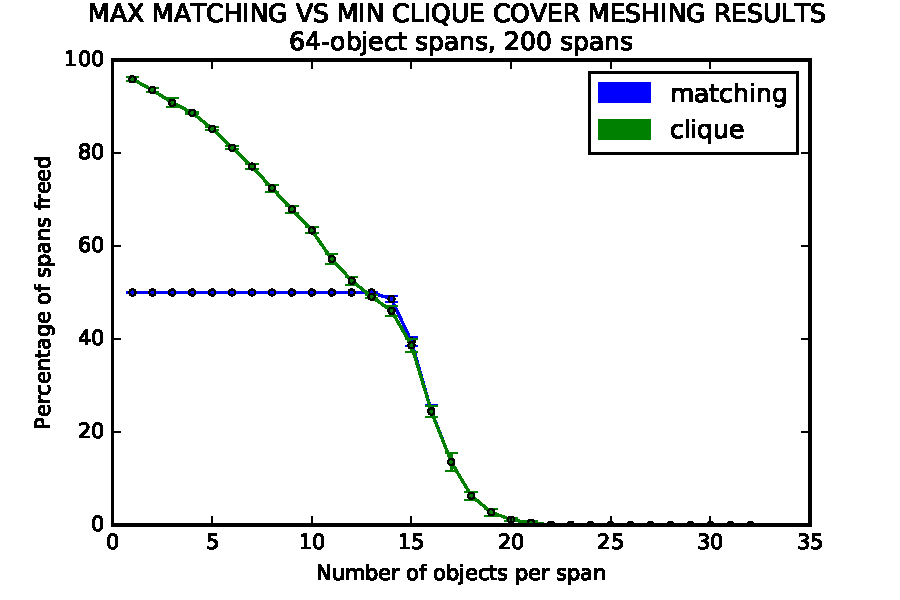
\includegraphics[scale = 1]{Chapters/mesh/figures/const_match_comp.pdf}
\centering
\caption{\textbf{Min Clique Cover and Max Matching solutions converge.} The average size of Min Clique Cover and Max Matching for randomly generated constant occupancy meshing graphs, plotted against span occupancy.  Note that for sufficiently high-occupancy spans, Min Clique Cover and Max Matching are nearly equal.}
\label{plot:const}
\end{figure}



When we instead assume bits are 1 independently with probability p, we expect the graph to have many more triangles.  For $p = r/b = 10/32, n = 1000$, the expected number of triangles is roughly 36,000.  However, we can see experimentally that these graphs behave quite similarly in Figure~\ref{plot:indep}.


\begin{figure}[h]
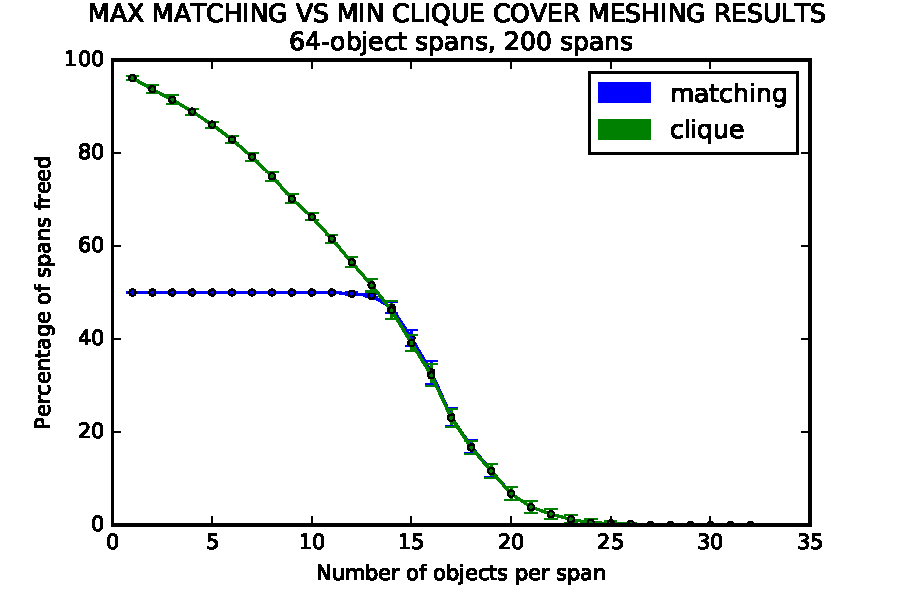
\includegraphics[scale = 1]{Chapters/mesh/figures/ind_match_comp.pdf}
\centering
\caption{\textbf{Converge still holds for independent bits assumption.} The average size of Min Clique Cover and Max Matching for randomly generated constant occupancy meshing graphs, plotted against span occupancy.  Note that for sufficiently high-occupancy spans, Min Clique Cover and Max Matching are nearly equal.}
\label{plot:indep}
\end{figure}

While constant occupancy graphs are fairly regular, independent bit graphs may not be.  Since strings have different occupancies, nodes which correspond to strings with relatively low occupancy will tend to have significantly higher degree than other nodes in the graph.  Meanwhile, other nodes may have strings with high occupancy, and therefore only have a few edges (probably with low-occupancy nodes).  So while there are many triangles, when the graph is sparse enough, even meshing cliques of size 3 and 4 will likely "abandon" adjacent high-occupancy nodes, one of which could have been matched with the high degree node to yield the same number of releases.

So in this case we still expect finding the maximum matching to be good enough.
% \paragraph{We Can Restrict Our Attention to Matching.}
\begin{comment}
The above analysis leads us to conclude that, since there are
relatively few triangles in meshing graphs, we can achieve almost the
full benefits of solving \textsc{MinCliqueCover} by only solving
\textsc{Matching}.
\end{comment}


\subsection{Theoretical Guarantees}
\label{subsec:analysis}
Since we need to perform meshing at runtime, it is essential that our
algorithm for finding strings to mesh be as efficient as possible. It
would be far too costly in both time and memory overhead to actually
construct the meshing graph and run an existing matching algorithm on
it. Instead, the \sm algorithm (shown in Figure \ref{fig:meshalg})
performs meshing without the need for explicitly constructing the
meshing graph.

For further efficiency, we need to constrain the value of the
parameter $t$, which controls \Mesh{}'s space-time tradeoff. If $t$
were set as large as $n$, then \sm could, in the worst case,
exhaustively search all pairs of spans between the left and right
sets: a total of $n^2/4$ probes.  In practice, we want to choose a
significantly smaller value for $t$ so that \Mesh{} can always
complete the meshing process quickly without the need to search all
possible pairs of strings.


\begin{lemma}
Let $t=k/q$ where $k>1$ is some user defined parameter and $q$ is the global probability of two
spans meshing. \sm finds a matching
of size at least $n(1-e^{-2k})/4$ between the left and right span sets
with probability approaching 1 as $n\geq 2k/q$ grows.
\end{lemma}

\begin{proof}
%\sm in essence creates a bipartite meshing graph by splitting the span set in half.
Let $S_l=\{v_1, v_2, \ldots v_{n/2}\}$ and $S_r=\{u_1,
u_2, \ldots u_{n/2}\}$. Let $t=k/q$ where
$k>1$ is some arbitrary constant. For $u_i\in S_l$ and $i \leq j \leq
j+t$, we say $(u_i,v_j)$ is a \emph{good match} if all the following
properties hold: (1) there is an edge between $u_i$ and $v_j$, (2)
there are no edges between $u_i$ and $v_{j'}$ for $i\leq j'<j$, and
(3) there are no edges between $u_{i'}$ and $v_{j}$ for $i< i'\leq j$.

We observe that \sm finds any good match, although it may
also find additional matches. It therefore suffices to consider only
the number of good matches. The probability $(u_i,v_j)$ is a good
match is $q(1-q)^{2(j-i)}$ by appealing to the fact that the collection of edges under consideration is acyclic. Hence, $\Pr(u_i \mbox{ has a good match})$
is
\begin{align*}
r:= q \sum_{i=0}^{k/q-1} \lp 1-q\rparen ^{2i} = q \frac{1-(1-q)^{2k/q}}{1-(1-q)^2}
% \geq q \frac{1-e^{-2k}}{2q-q^2}
 > \frac{1-e^{-2k}}{2} \ .
\end{align*}

To analyze the number of good matches, define $X_i = 1$ iff $u_i$ has
a good match. Then, $\sum_i X_i$ is the number of good matches. By
linearity of expectation, the expected number of good matches is
$rn/2$. We decompose $\sum_i X_i$ into \[Z_0+Z_1+\ldots + Z_{t-1} ~~\mbox{
  where }~~ Z_{j} = \sum_{i\equiv j \bmod t} X_i \ .\] Since each
$Z_j$ is a sum of $n/(2t)$ independent variables, by the Chernoff
bound,\\ $P\lp Z_j < \lp 1-\epsilon \rparen E[Z_j]\rparen \leq \exp\lp -
\epsilon^2 r n/(4t)\rparen$.  By the union bound,
$$P\lp X < \lp 1-\epsilon \rparen rn/2\rparen \leq t \exp\lp - \epsilon^2 r
n/(4t)\rparen$$ and this becomes arbitrarily small as $n$ grows.
\end{proof}

In the worst case, the algorithm checks $nk/2q$ pairs. For our
implementation of \Mesh, we use a static value of $t = 64$; this value
enables the guarantees of Lemma 5.1 in cases where significant meshing
is possible.  As Section~\ref{sec:evaluation} shows, this value for
$t$ results in effective memory compaction with modest performance
overhead.




\subsection{New Lower Bound for Maximum Matching Size}
\label{subsec:lowerbound}

In this section, we develop a bound for the size of the maximum matching in a graph that can easily be estimated in the context of meshing graphs.  As meshing may be costly to perform, this lower bound is useful as it can be used to predict the magnitude of compaction achievable before committing to the process.  In the case where little compaction is possible, it is often better not to try to mesh and instead conserve resources for other tasks. The quantity we introduce will always lower bound the size of  the maximum matching and will typically be relatively close to the size of the maximum matching.  For example, if we want to release 30\% of our active spans through meshing, but the bound suggests a release of less than 5\% is possible, we can infer that the maximum matching on the graph is small and meshing is currently not worth attempting.

Our approach is based on extending a result by McGregor and Vorotnikova \cite{McGregorV16}. Let $\ndegree(u)$ be the degree of node $u$ in a graph. They considered the quantity
$\sum_{e\in E} 1/\max(\ndegree(u),\ndegree(v))$
and showed that it is at most a factor $3/2$ larger than the maximum matching in the graph and at most a factor $4$ smaller in the case of planar graphs. These bounds were tight.  For example, on a complete graph on three nodes, the quantity is $3/2$ while $M$ is 1. Meshing graphs are very unlikely to be planar but are likely be almost regular, i.e., most degrees are roughly similar.
We need to extend the above bound such that we can guarantee that it never exceeds the size of the maximum matching while also being a good estimate for the graphs that are likely to arise as meshing graphs.

%\begin{theorem}
%Define $W(G)$ to be a fractional matching on graph $G = (V,E)$ such that $$W = \sum_{(u,v) \in E} \min\lp %\frac{1}{\ndegree\lp u\rparen },\frac{1}{\ndegree\lp v\rparen }\rparen $$
%Then $W\leq \frac{3}{2} M$ where $M$ is the cardinality of the maximum matching on $G$.
%If $G$ is bipartite, then $W \leq M$.
%\end{theorem}

%For general graphs, $W$ is not always a lower bound on the maximum matching (hence the need for the $\frac{3}{2}$ factor).  For example, on a complete graph on three nodes, $W$ is $\frac{3}{2}$ while $M$ is 1.

%\begin{figure}[h]
%\includegraphics[scale = .7]{figures/triangle_matching.png}
%\centering
%\caption{W is not a lower bound for the maximum matching on a triangle.}
%\end{figure}
One simple approach is to scale the above quantity by a factor of $2/3$,
but this can result in a poor approximation for the size of the
maximum matching for some graphs of interest. Instead, we take a more
nuanced approach. Specifically, we prove the following theorem (proof omitted
due to space constraints):
%in the
%Appendix:

%While it is tight for this example, for larger non-bipartite graphs it seems like scaling $W$ down by %$\frac{2}{3}$ is overkill.  For instance, for a complete graph on an odd number of nodes k, $W = %{{k}\choose{2}} \frac{1}{k-1} = \frac{k}{2}$, while $M = \frac{k-1}{2}$.
%The following theorem provides a tight lower bound for this example.


\begin{theorem}
\[
\W=\sum_{e\in E} \frac{1}{\max(\ndegree(u), \ndegree(v))+I[\min(\ndegree(u),\ndegree(v))>1]}\leq M \ .
\]
%where $f(1,\cdot)=f(\cdot,1)=f(2,3)=f(3,2)=0$ and $f(\cdot,\cdot)=1$ otherwise. Then, $\sum_{e\in E} w_e \leq M$.
% . Then, $\sum_{e\in E} w_e \leq M$.
\end{theorem}

\begin{proof}
We begin by showing that the simpler quantity $W$ is a lower bound of the maximum matching $M$.
\[
W = \sum_{e\in E} \frac{1}{\max(\ndegree\lp u\rparen, \ndegree\lp v\rparen )+1}\ .
\]
%For each edge $e = (u,v) \in G$, define $\W$$(e)=min\lp \frac{1}{\ndegree\lp u\rparen +1},\frac{1}{\ndegree\lp %v\rparen +1}\rparen$.  L
Let $U$ be an arbitrary set of $t$ nodes in $G$ where $t$ is odd.   Define $$W(U) = \sum_{u,v \in U} \frac{1}{\max(\ndegree\lp u\rparen, \ndegree\lp v\rparen )+1} \ . $$ As a corollary of Edmonds Matching Polytope Theorem, it can be shown that $W \leq M$ if  $W(U) \leq (|U|-1)/2$. We can argue this as follows:

\begin{align*}
W(U) &= \sum_{(u,v) \in U} \min \left(\frac{1}{\ndegree(u)+1},\frac{1}{\ndegree(v)+1}\right )\\
& \leq \sum_{(u,v) \in U}\frac{1}{2}\lp \frac{1}{\ndegree\lp u \rparen +1}+\frac{1}{\ndegree\lp v\rparen +1}\rparen\\
&\leq \sum_{(u,v) \in U}\frac{1}{2}\lp \frac{1}{\ndegree_U\lp u\rparen +1}+\frac{1}{\ndegree_U\lp v\rparen +1}\rparen\\
&= \frac{1}{2} \sum_{u \in U} \frac{\ndegree_U\lp u\rp }{\ndegree_U\lp u\rp +1} \leq  \frac{1}{2} \lp \frac{t-1}{t}\rp  t = \frac{t-1}{2}
\end{align*}
where $\ndegree_U(u)$ in the number of neighbors of $u$ in the set $U$.
The second line follows from the fact that the minimum of two quantities is bounded above by their average.  The third line follows from the fact that the degree of any node in a subgraph is bounded above by its degree in the original graph.  The fourth line follows from summing over nodes instead of edges, and then reasoning that in the worst case U is a clique and so $\degree_U(u) = t-1$ for all u $u$.

\iffalse
Recall that we prove in Section~\ref{subsec:lowerbound} that when
\[
w_e=\min\lp \frac{1}{\ndegree\lp u\rp+1 },\frac{1}{\ndegree\lp v\rp+1 }\rp
~~\mbox{ and }~~\W=\sum_{e\in E} w_e \ .\]
then $\W$ is a lower bound on the cardinality of the maximum matching M(G).
\fi


In some cases $W$ is too conservative; it assigns little weight to edges which it could safely have assigned much more.  For example, if $e$ is isolated (meaning its endpoints have degree 1), $W(e) = 1/2$.  However, it is always safe to assign weight 1 to $e$, since $M(G-e) = M(G)-1.$  If we modified our rule for $W$ so that for any edge $e= (u,v)$ s.t. $\deg(u)=\deg(v) = 1$ we assigned weight $ \min(1/\deg(u),1/\deg(v))$ instead of $ \min(1/\deg(u)+1,1/\deg(v)+1)$, we would always assign weight 1 to isolated edges.

In fact, a more general rule is true.  For any edge $e= (u,v)$, if either $\deg(u) or \deg(v) = 1$ then we may assign it weight $\min(1/\deg(u),1/\deg(v))$.

\iffalse
At this point it is natural to ask whether we can remove the $+1$s from the denominator for other edges.  We cannot of course do so for $\deg(u) = \deg(v) = k >1, k \in 2\mathbb{Z}$ since for a clique on k+1 nodes this rule would result in total weight $(k+1)/2$.\\

However, we can remove the $+1$ under certain circumstances. We show that if one of the endpoints has degree one then this is the case.
\fi

%prove several rules of this form.  For each rule we specify values of $\deg(u)$ and $\deg(v)$ for which the %$+1$ can be removed from the denominator of the edge weight.
%First we restate the claim that isolated edges may safely be assigned weight 1.
%\begin{lemma}
%Define $\W(G)$ as follows:\\
%For each $(u,v) \in G$,\\
%if $\deg(u) = \deg(v) = 1$, $\W(u,v) =  \min(\frac{1}{\deg(u)},\frac{1}{\deg(v)})$.\\
%else $\W(u,v) =  \min(\frac{1}{\deg(u)+1},\frac{1}{\deg(v)+1})$.
%Then $\W(G) \leq M(G)$.
%\end{lemma}
%\begin{proof}
%Already proven above.
%\end{proof}
%Next we will amend $\W$ to include the following rule: when one endpoint has degree 1 and the other has %degree k, assign weight $\frac{1}{k}$.

Define $\W$ as follows:
\[\W=\sum_{(u,v)\in E} \W(u,v) \]
where
\[
\W(u,v)=\frac{1}{\max(\ndegree\lp u\rp, \ndegree\lp v\rp )+I[\min(\ndegree(u),\ndegree(v))> 1]}\]

We now show that $\W \leq M$. We have proven that $W(U)\leq (t-1)/2$ on any odd-size subgraph $U$, $|U| = t$.  Define subsets $U_1$ and $U_2$ of $U$ such that $U_1 \cup U_2 = U$.  $U_1$ is the set of all nodes in $U$ of degree 1 and all nodes in $U$ adjacent to a node of degree 1, and $U_2$ is the set of all other nodes in $U$.  Let $G(U_2)$ denote the subgraph of $U$ induced by $U_2$, and let $|U_1| = x$ where x is even.  Then $W(G(U_2)) = \W(G(U_2)) \leq (t-x-1)/2$.  So to complete our proof we must show that all remaining edges (call them $E'$) have total weight $\leq x/2$.

Assume WLOG that there are no isolated edges in $G$ (if there are, we can group them with $G(U_2)$ and retain the $(t-x-1)/2$ bound).

\begin{align*}
\W(E') & \leq \frac{1}{2} \sum_{u,v \in E'} \lp \frac{1}{\deg(u)}+\frac{1}{\deg(v)}\rp\\
& = \mathlarger{\sum_k} \Big(\sum_{v \in U_1, \deg(v) = k} \frac{\delta}{k} + \frac{k-\delta}{2(k+1)}\Big)
\end{align*}
where $\delta$ denotes the number of degree 1 nodes adjacent to $v$.\\
Let $f(\delta) = \delta/k + (k-\delta)/(2(k+1))$.  We are interested in finding the maximum value $f(\delta)/(\delta+1)$ can take on; if it can never take a value greater than $1/2$ then $\W(E')$ cannot be greater than $x/2$.
$$\frac{\partial\frac{f(\delta)}{\delta+1}}{\partial \delta} = \frac{2-k}{2k(\delta+1)^2}$$
which is always negative for $k \geq 2$.  So, $f(\delta)/(\delta+1)$ is maximized at $\delta = 0$, so  $f(\delta)/(\delta+1) \leq k/(2(k+1)) < 1/2.$

There is one final detail we have not considered: $x$ might be odd.  In this case, $|U_2|$ is even and we can't appeal to Theorem 3 to say that $\W(G(U_2)) \leq (t-x-1)/2$.  However, we can simply remove one node $\node'$ from $U_2$; the resulting odd-size subgraph has weight at most $(t-x-2)/2$.  Since $\W$ is a valid fractional matching, the weight assigned to all edges adjacent to $\node'$ cannot exceed 1, so we can say that $\W(G(U_2)) \leq (t-x)/2$.  Now we must show that $\W(E') \leq (x-1)/2$.

We have shown that the edge weight per node in $U_1$ cannot exceed $1/2$.  $\W(E')$ is minimized when there is exactly 1 node of degree 1, with a degree k neighbor. In this case, the only edge in $E'$ will be assigned weight $k/(2(k+1))< 1/2$.  $\W(E') \leq 1/2 + (x-2)/2 = (x-1)/2$ and the theorem is proven.
\end{proof}


\paragraph*{A remark on estimating $\W$.}  If we wish to use this lower bound to decide whether to begin meshing by predicting the size of the maximum matching, we cannot compute it exactly because we do not know the degrees of the nodes in the graph.  However, we do know the degree distribution of the graph and so it is possible to calculate the expected value of $\W$.





%\subsection{Summary}
%\label{subsec:theorysummary}

\subsection{Summary of Analytical Results}
We show the problem of meshing is reducible to a graph problem,
\textsc{MinCliqueCover}.  While solving this problem is infeasible, we
show that probabilistically, we can do nearly as well by finding the
maximum \textsc{Matching}, a much easier graph problem. We analyze our
meshing algorithm as an approximation to the maximum matching on a
random meshing graph, and argue that it succeeds with high
probability.  Finally, we prove a new lower bound on the maximum matching for graphs based on degree distribution.
As a corollary of these results, \Mesh breaks the Robson
bounds with high probability.

%for a broad class of applications.
%As long as programs do not alter
%programs that do not alter their allocation behavior in response to
%addresses the allocator returns.


\begin{comment}
  An adversary attempting to create an
unmeshable memory state requires the capability to position objects at
the same locations in multiple spans.  But an address-oblivious
adversary can only do this with low probability - since allocation
offsets within a span are random, the best it can do is free some
objects from each span and hope that some of the remaining objects
reside at the same offset.  Since objects are distributed uniformly at
random from within spans, our analytical results hold and therefore
there is either a large maximum matching on the resulting meshing
graph (indicating significant compaction is possible) or spans are so
full that fragmentation is not significant.
\end{comment}
